\documentclass[12pt]{extarticle}
\usepackage[utf8]{inputenc}
\usepackage{ebgaramond}
\usepackage[export]{adjustbox}
\usepackage{eso-pic, graphicx}
\usepackage[margin=0.5in]{geometry}
\geometry{
  paperheight=8.5in,
  paperwidth=5.5in,
  heightrounded,
}
\usepackage{setspace}

\usepackage{pgfornament}

\usepackage{subcaption}

\usepackage{verse}
\newcommand{\attrib}[1]{%
\nopagebreak{\raggedleft\footnotesize #1\par}}
\renewcommand{\poemtitlefont}{\normalfont\large\itshape\centering}

\pagenumbering{gobble}
\setlength\parindent{0pt}

\newcommand\AtPageUpperRight[1]{\AtPageUpperLeft{%
 \put(\LenToUnit{\paperwidth},\LenToUnit{0\paperheight}){#1}%
 }}%
\newcommand\AtPageLowerRight[1]{\AtPageLowerLeft{%
 \put(\LenToUnit{\paperwidth},\LenToUnit{0\paperheight}){#1}%
 }}%
\setlength{\parskip}{2em}

\begin{document}
\topskip0pt
\vspace*{\fill}

\begin{figure}[h!]
\centering
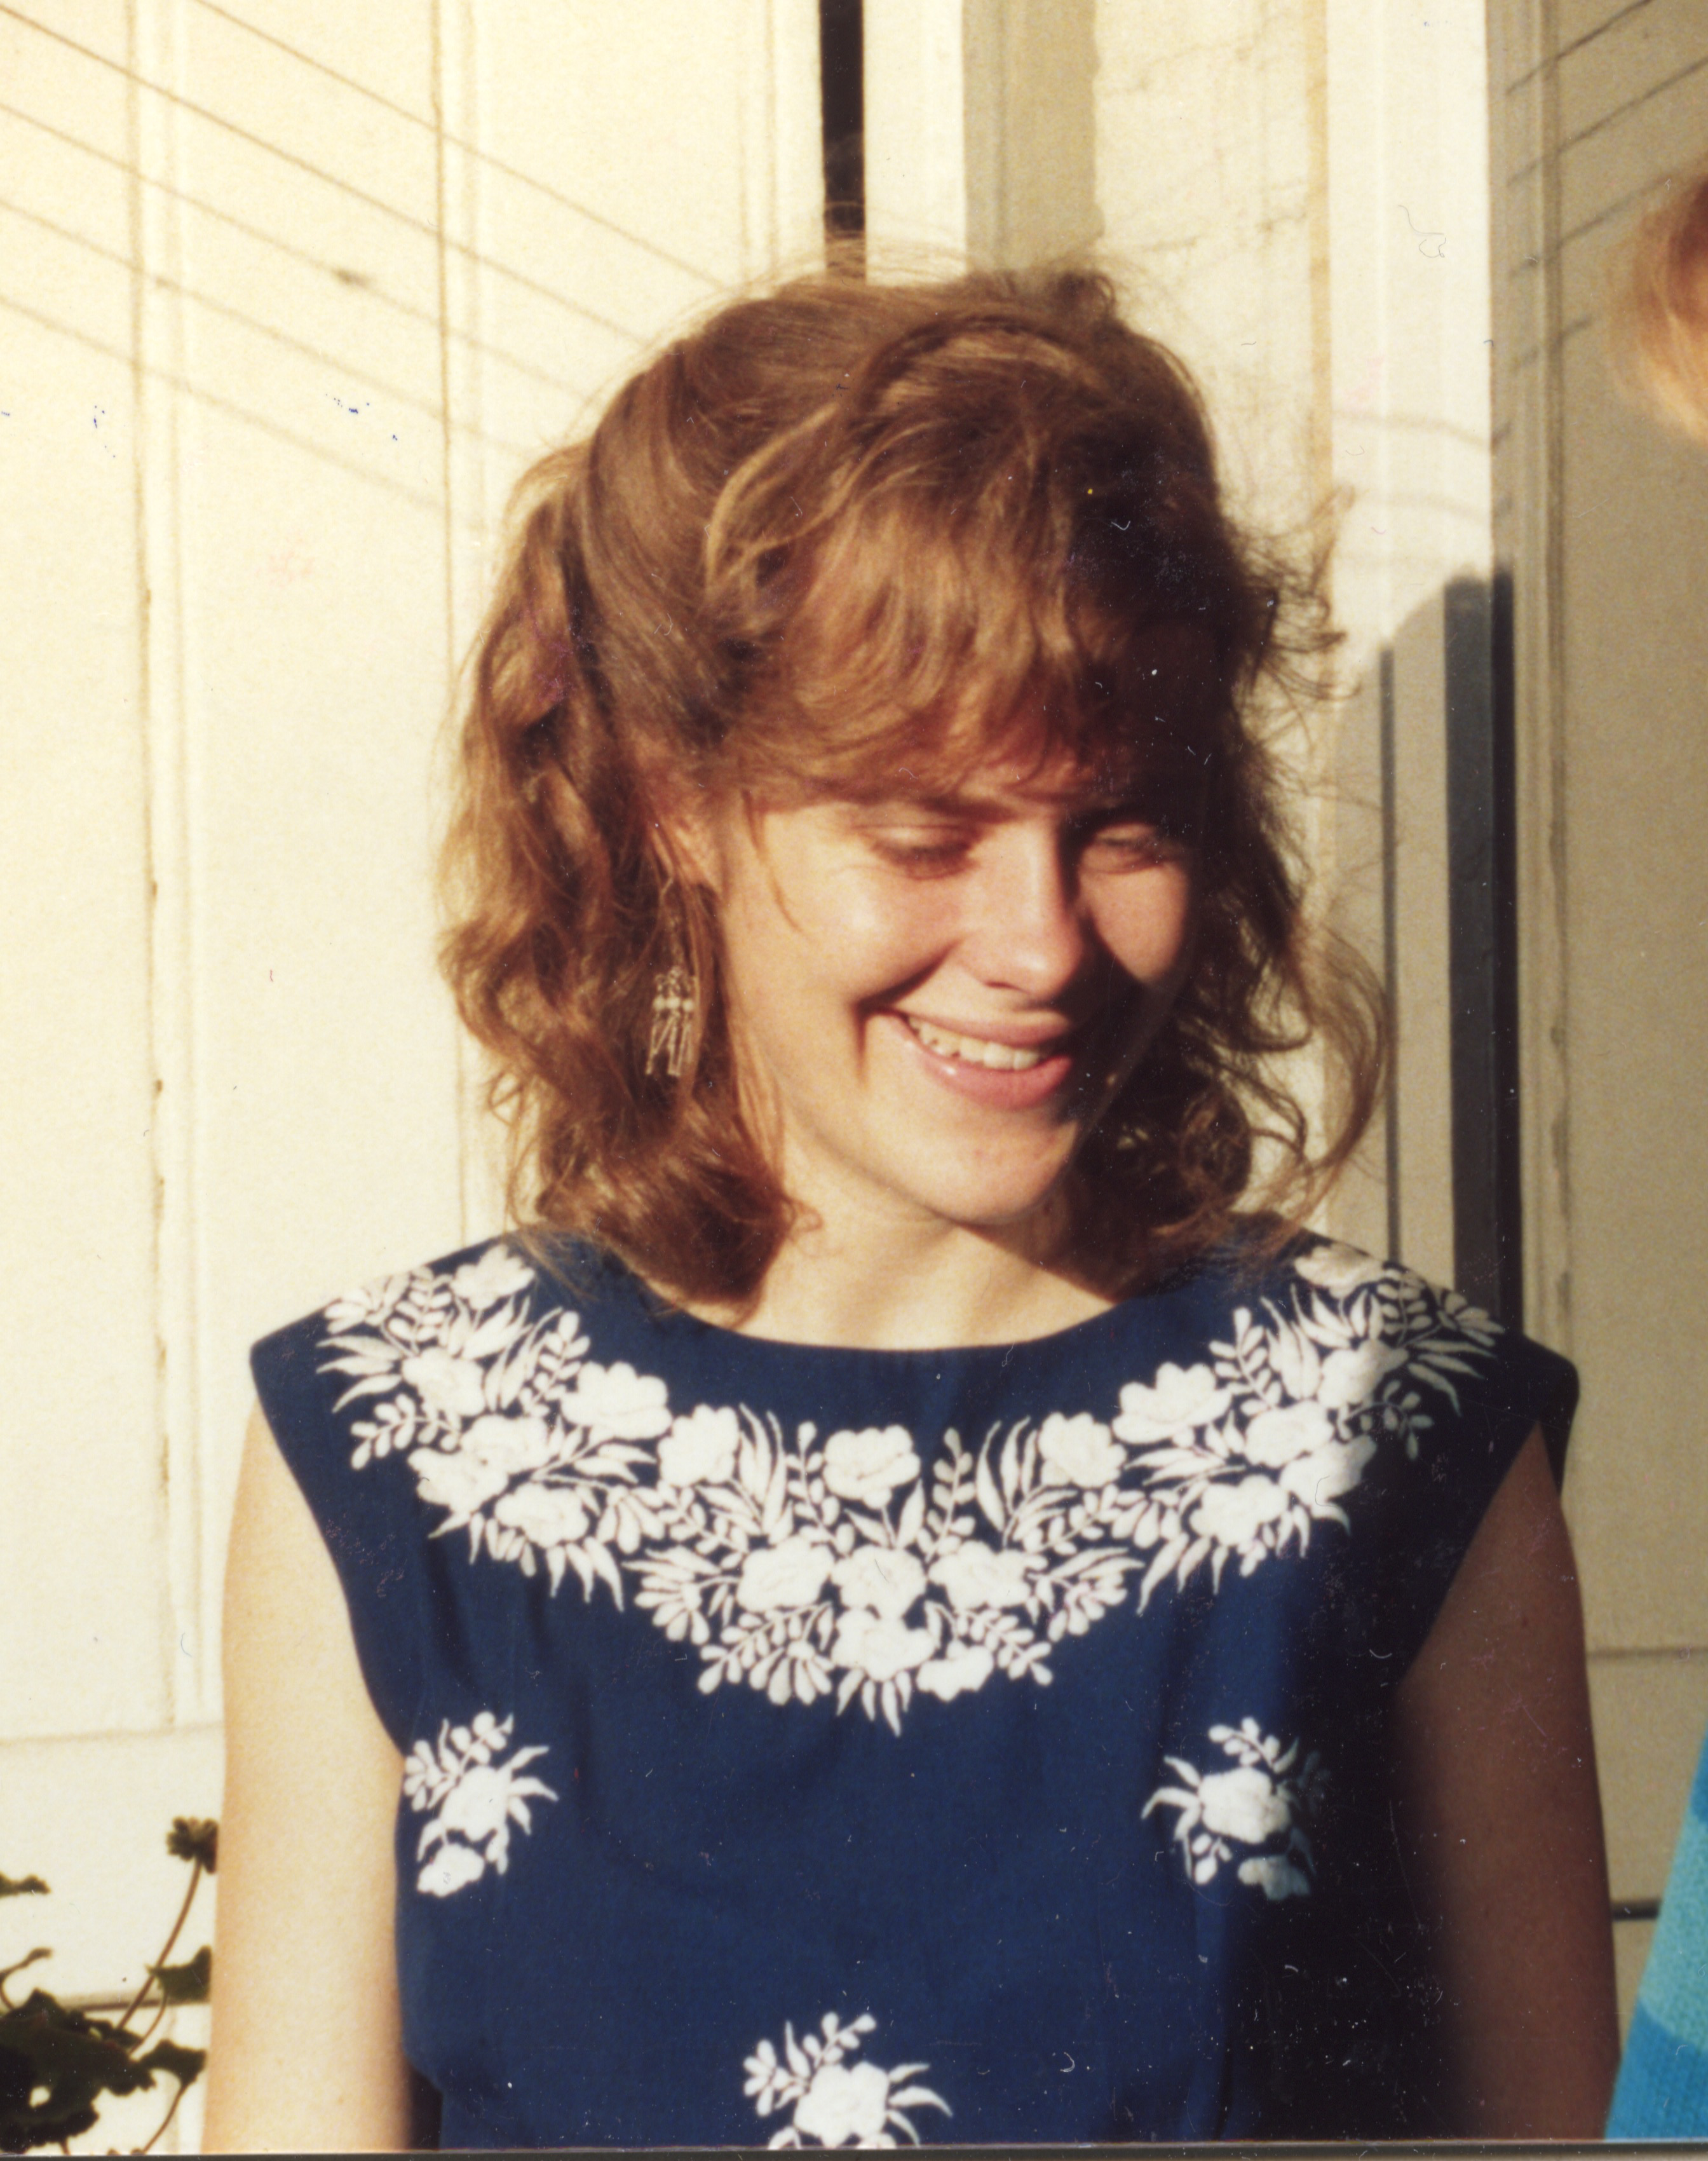
\includegraphics[width=9cm]{pg1.png}
\end{figure}

\begin{center}
\pgfornament[width = 9cm, anchor=center, ydelta=0pt]{88}
\end{center}

{\centering \huge Deborah Lee Simmons\par}
{\centering \Large October 2 1962 - October 28 2022\par} 

\vspace*{\fill}

% Base ornaments in corners
\AddToShipoutPictureBG*{%
   \AtPageUpperLeft{\put(0,-21){\pgfornament[width=1.5cm]{61}}}
   \AtPageUpperRight{\put(-42,-21){\pgfornament[width=1.5cm,symmetry=v]{61}}}
   \AtPageLowerLeft{\put(0,21){\pgfornament[width=1.5cm,symmetry=h]{61}}}
   \AtPageLowerRight{\put(-42,21){\pgfornament[width=1.5cm,symmetry=c]{61}}}
}

% \AddToShipoutPictureBG*{%
%    \AtPageUpperLeft{\put(30,-51){\pgfornament[width=1.5cm]{61}}}
%    \AtPageUpperRight{\put(-72,-51){\pgfornament[width=1.5cm,symmetry=v]{61}}}
%    \AtPageLowerLeft{\put(30,51){\pgfornament[width=1.5cm,symmetry=h]{61}}}
%    \AtPageLowerRight{\put(-72,51){\pgfornament[width=1.5cm,symmetry=c]{61}}}
% }

\newpage
\topskip0pt
\vspace*{\fill}
Deborah Lee Simmons was born in Ajo, Arizona, in 1962, to Hilah (teacher) 
and Norman (biologist) Simmons. Followed two and a half years later by
brother David, she began her teaching career early with this new sibling
who, though not the best student, thrived under her tutelage. It was not
long before she started `organizing' her family. We were an unruly lot
but that did not stop her from trying.

In `66 the family packed the station wagon and moved to Ft. Smith in the
Northwest Territories, an idyllic little town on the banks of the Slave
River. Early formative experiences include the summers spent on the
banks of the Keele River in the Mackenzie Mountains where Deb was first
introduced to the Northern ``bush''. Norman was doing research on Dall
Sheep for the Canadian Wildlife Service supported by three Mountain Dene
families from Tulita, a town on the Mackenzie River. Their guidance was
essential to the success of his research, providing expert knowledge on
the land, its wildlife and its people. The Simmons clan was treated like
family and had the unique opportunity to learn about the traditional
skills, stories and philosophies of the Sahtú Dene. These experiences
likely inspired what would ultimately become Deborah's mission in the
North, namely to support and strengthen Dene culture, language, and
self-governance; and to ensure the participation of the Dene people in
the management of their natural resources.

The year 1973 brought her brother Daniel into the fold. In 1975 the
Simmons family moved further north to Yellowknife on the shore of Great
Slave Lake and a few months later her sister Sarah was born.

\AddToShipoutPictureBG*{%
   \AtPageUpperLeft{\put(18,-72){\pgfornament[width=1.5cm]{41}}}
   \AtPageUpperRight{\put(-61,-72){\pgfornament[width=1.5cm,symmetry=v]{41}}}
   \AtPageLowerLeft{\put(18,60){\pgfornament[width=1.5cm,symmetry=h]{41}}}
   \AtPageLowerRight{\put(-61,60){\pgfornament[width=1.5cm,symmetry=c]{41}}}
}

\vspace*{\fill}

\newpage
\topskip0pt

\vspace*{\fill}

During this time, Deb distinguished herself both as a top student and
through her many extra-curricular interests such as cross country
skiing, camping, and canoeing, the latter a favorite family activity.
Her mother Hilah surrounded the family with music and Deb learned piano
and played french horn, then flute, in the Sir John Franklin High School
band. Between these pursuits she could almost always be found with a
book in hand. She was an absolutely voracious reader. In school, Deb
befriended the quirky, talented and interesting kids, a trait that would
continue throughout her life as evidenced by her sprawling network of
unique individuals. Her love of languages inspired her to do a French
immersion semester in Caraquet, New Brunswick. At graduation, Deb was
second in her class and selected as Valedictorian.

Deb's post-secondary career was the ground of her true flowering as a
thinker, writer, activist, and teacher. She was a committed socialist
with a vision to build a just society for all by advancing and
amplifying the voices of the dispossessed. Following the completion of
her PhD Dissertation on the political economy of Indigenous resistance
in the Social and Political Thought program at York University in
Toronto, she went on to teach at the University of Manitoba.

After this stint in academia, Deb returned to her childhood roots with a
job as a social science researcher in the Sahtú region, working with
some of the same families that her father had worked with decades
before. Picking up the baton from him, she advocated for the full
participation of the Dene in conservation and land management. Her
principled commitment to indigenous self-determination brought her,
ultimately, to the position of Executive Director of the Sahtú Renewable
Resources board. In this role, she was able to effect lasting change,
notably by having the co-management of natural resources recognized as a
right within the framework of land claims agreements. Along with her
tireless struggle to have indigenous rights recognized by the legal
authorities that would rule the land, she championed Dene ways of
knowing and being, namely by integrating Dene language and oral
histories through all projects in which she was involved.

Her colleagues within academic, professional, and activist circles have
spoken beautifully of Deb's tireless work ethic, commitment to her
ideals and innate good nature (see below). Her capacity to organize and
network, along with her joyous and kind spirit, drew many to her. Though
always gentle, she was never deterred. This magnetic energy surely
emanated from her huge heart.

Deborah was a pillar of her family and will be sorely missed. She is
survived by her mother Hilah, her partner Morris, her siblings and their
children. She was a fun and loving auntie not only to Ruby and Sadie,
(Sarah), and Noah, Hilah and Remi (Danny), but also to Morris' niece
Jennie and to many young people in the Sahtú on whom she made a lasting
impact. In her life, cut far too short, Debby passionately planted many
seeds that already are blooming. May she be remembered not only for her
legacy but for the irrepressible joy and passion she brought to bear
throughout her life.

% \begin{center}
% \pgfornament[width = 3cm, anchor=center, ydelta=0pt]{72}
% \pgfornament[width = 3cm, anchor=center, ydelta=0pt]{75}
% \pgfornament[width = 3cm, anchor=center, ydelta=0pt]{73}
% \end{center}

% \vspace{0.5cm}


% \begin{center}
% \pgfornament[width = 9cm, anchor=center, ydelta=0pt]{88}
% \end{center}

\vspace*{\fill}

% \AddToShipoutPictureBG*{%
% 	\AtTextLowerLeft{%
% 		\raisebox{.5\textheight}{%
% 			\hspace*{.5\textwidth}%
% 			\makebox[0pt]{\includegraphics[width=1.1\textwidth, height=1.05\textheight, valign=c]{pg3-bg.png}}%
% 		}%
% 	}%
% }

\vspace*{\fill}

\clearpage
\topskip0pt
\vspace*{\fill}

% \poemtitle{To Those I Love and To Those Who Love Me}

% \settowidth{\versewidth}{I give you my love, for you can only guess}
% \begin{verse}[\versewidth]
% {\setstretch{1.6}
% When I am gone, release me, and let me go;\\
% I have so many things to see and do.\\
% You mustn't tie yourself to me with tears,\\
% Be happy we had so many years.\\
% I give you my love, for you can only guess \\
% How much you gave to me in happiness.\\
% I thank you for the love you have shown,\\
% But now it's time I travel alone.\\
% So grieve a while for me, if grieve you must,\\
% Then let your grief be comforted by trust.\\
% It's only for a while that we must part\\
% So bless the memories within your heart.\\
% I won't be far away for life goes on,\\
% So if you need me, call me, and I will be near.\\
% And if you listen with your heart, you'll hear\\
% All my love around you, soft and clear.\\
% And when you must come this way alone\\
% I'll greet you with a smile and ``Welcome Home.''\\
% }
% \end{verse}

\AddToShipoutPictureBG*{%
   \AtPageUpperLeft{\put(30,-51){\pgfornament[width=1.5cm]{61}}}
   \AtPageUpperRight{\put(-72,-51){\pgfornament[width=1.5cm,symmetry=v]{61}}}
   \AtPageLowerLeft{\put(30,51){\pgfornament[width=1.5cm,symmetry=h]{61}}}
   \AtPageLowerRight{\put(-72,51){\pgfornament[width=1.5cm,symmetry=c]{61}}}
}

\vspace*{\fill}

\end{document}
